\documentclass[12pt]{thesis} %%%%%%%%%%%%%%%%%%%%%%%%%%%%%%%%%%%%%%%%%%%%%%%%%%
\usepackage[utf8]{inputenc}

\newcommand{\autor}{Nils der Typ} % Vor und Nachname / GivenName FamilyName (The one on your matriculation)
\newcommand{\matrikel}{007}	% Matrikel / Matriculation number
\newcommand{\erstgutachter}{Prof. Dr.-Ing. Timo Gerkmann} % Erstgutachter / Primary Reviewer
\newcommand{\zweitgutachter}{Dr.-Ing. Martin Krawczyk-Becker} % Zweitgutachter / Secondary Reviewer
% \newcommand{\betreuer}{Name Betreuer} % Betreuer  delete / comment this line if you didn't have a supervisor or the supervior is one of the reviewers
\newcommand{\arbeitstitel}{Real-Time Capable Yo Mama} % Titel angeben / title of your thesis
\newcommand{\arbeitstyp}{Bachelor Thesis} %Typ angeben / type of the thesis 
\newcommand{\studycourse}{Informatik} % Studiengang/ study course
% \newcommand{\german}{ngerman}% delete / comment this line for English

\usepackage{hcisty}

\usepackage{todonotes}
\usepackage{amsmath}
\usepackage{algorithm}
\usepackage[noend]{algpseudocode}
\usepackage{booktabs}


% WORDS THAT SHOULD NOT BE HYPHENATED
\hyphenation{GMMDNN}
\hyphenation{VTLN}
\hyphenation{DNN}
\hyphenation{MLP}
\hyphenation{GMM}




\start{1}{1}
% \start[1]{1} <= show both abstracts
% \start[0]{1} only german. \start[1]{0} only english .\start[0]{0} nothing
% change the abstract.tex and abstractGER.tex to your needs
\newpage\chapter{Introduction}
\label{chapter:introduction}




\newpage\chapter{Basics}
\label{chapter:basics}

\section{Loudness}

Including the human perception in the algorithm is a complex task as for example absolute threshold of hearing and the subjective perception of sound pressure are varying for different frequencies (see Fig. \ref{LDNSGraph}).\\

\begin{figure}[H]
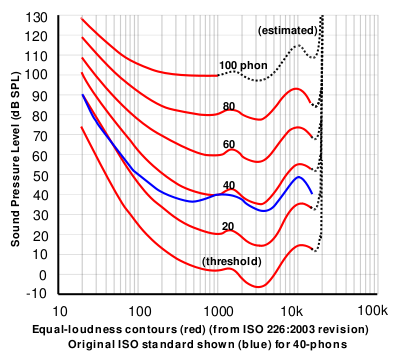
\includegraphics[width=0.5\textwidth]{images/loudnessGraph}
	\centering
	\caption{Loudness perception\cite{wikiLoud}}
	\label{LDNSGraph}
\end{figure}

While gathering information on how to improve the plug-in in terms of human perception the ITU-R BS.1770-4\cite{ITUalgo} algorithm was evaluated. This algorithm classifies an audio file for its humanly perceived loudness. It is mainly used by television and music streaming services as the program loudness can be kept steady while switching content. As the perception is of substantial interest for mixing a song, this was investigated in this study. Due to a good documentation about how to implement the loudness algorithm a copy of it was build in Python and it was decided which elements to be adopted in the plug-in. The first and second element were two filters. Their use is to mimic the human perception of sound pressure at different frequencies. The first filter is a low cut for the reason that human hearing is insensitive to low frequencies. The second filter is a high shelf and is ‘\textit{used to account for the acoustic effects of the head}’\cite{ITUalgo}. This imitation of the human hearing is substantially simplified but cost-effective in terms of computation. The low cut filter has a cutoff frequency of 38 Hz, the high shelf of around 1681 Hz.\\

\begin{figure}[H]
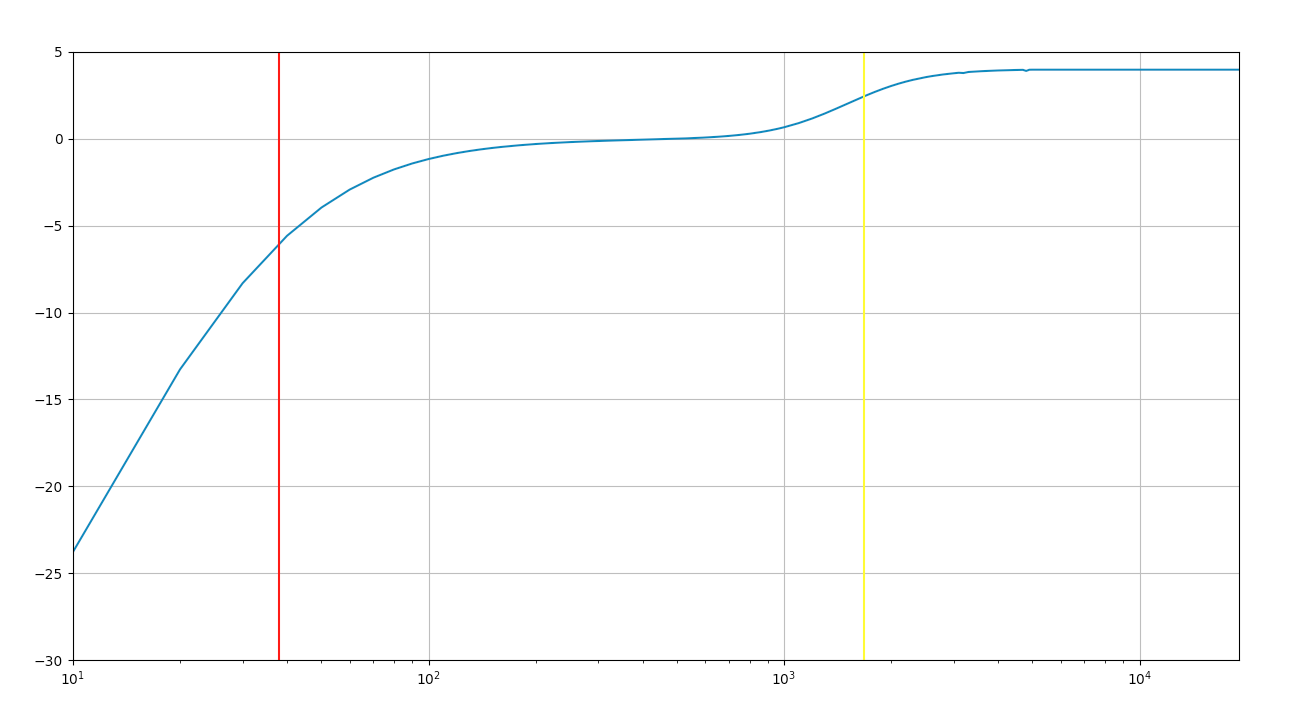
\includegraphics[width=0.8\textwidth]{images/filter_test}
	\centering
	\caption{Plotted outcome of adopted filter implementation for the audible spectrum of frequencies}
	\label{filterTest}
\end{figure}

The filter section is followed by the determination of a root mean square (RMS) value for time windows of 400ms overlaping 75\% (a value is saved every 100ms). This means it is calculating the root of the average from the squares of each sample in the set time window which equals the power of the signal.\\
RMS calculation is used because it is part of the imitation of human perception: a human will not interpret a small impulse of a handful of samples as loud as a audio signal at the same level of longer duration.  For example ‘\textit{a 3-msec pulse must have a level about 15 dB higher to sound as loud as a 0.5-sec (500-msec) pulse}'\cite{masterHA}.\\
Subsequently, all RMS values below a absolute threshold of -70LKFS\footnote{definition in \cite{ITUalgo}} are sorted out by a gate and a average value is determined. Another gate of -10LU below the average is applied on the rms values and a second averaging of measurements is performed. The resulting average is the loudness of the processed audio file.\\

\section{Vocal Rider}

'Vocal Rider' by Waves is a commercially available audio plug-in which realizes a automatic gain adaption for vocal signals.

\begin{figure}[H]
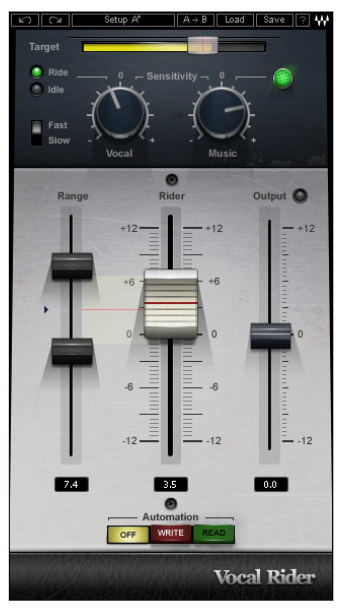
\includegraphics[width=0.35\textwidth]{images/vocalRiderUI}
	\centering
	\caption{UI of Waves 'Vocal Rider'\cite{vocalRiderM}}
	\label{VRUI}
\end{figure}

The vocal signal's level is adjusted to the set \textit{target} value (at top of Fig. \ref{VRUI}). The '\textit{target sets the reference range for vocal mix positioning. [It] (…) will move the Rider Fader’s ‘0’ calibration.}'\cite{vocalRiderM}. Additionally a user can control the maximal gain adaption with the '\textit{range}' slider and adjust the resulting level to the backtrack via a output gain. For results depending on the instrumental backtrack a side chain input can be used and adjusted with the '\textit{music}' potentiometer.\\
As in this study the same basic idea is realized with a independent approach it is possible to adopt useful results from the comparison (see chapter \ref{chapter:comparison}) of both plug-ins and remain with potential advantages.\\

\section{Optimization}

For the comparison in chapter \ref{chapter:comparison} optimization methods were used to find parameters for the study plug-in to get to similar results as the 'Vocal Rider' does. Therefore the scipy\cite{scipy} methods scipy.optimize.brute and scipy.optimize.minimize were used.\\
Previously a function had to be written which returns the current problem as a number. Thereby a smaller number equals a smaller problem.\\
The '\textit{brute}' optimization algorithm '\textit{computes the function’s value at each point of a multidimensional grid of points, to find the global minimum of the function}'\cite{scipyB}. The according '\textit{grid}' is therefore previously defined for the current optimization problem. This is done by initializing a set of user defined bounds and step sizes for each of the parameters which a transferred to the function to be optimized.\\
The '\textit{minimize}' optimization algorithm per default '\textit{uses the L-BFGS-B algorithm ... for bound constrained minimization}'\cite{scipyM}. This algorithm is able to compute faster and more selective but needs a good inital parameter guess to get to a proper result.\\


\newpage\chapter{Approaches}
\label{chapter:approach}

\section{Overview}

The basic approach works in five steps: filter, root mean square (RMS) calculation, gate, gain adaption, delay.\\
It starts with a low-cut and a high-shelf filter which will be applied sample wise on the incoming audio. Those filters are a simplified mapping of the perception of sound pressure for human beings. In this way (as done in FOOTNTE) it is the first step to adjust the plug-in to loudness instead of sound pressure. Although in the basic approach the plug-in will not be working with the full loudness detection algorithm (FUTNOT) due to calculation time and real time capability (see SPÄTER? oder hier?).\\
After the filter section every sample is passed to the RMS calculation.  This will output the squared average of a previously specified period of time. The determination of the square root is not necessary because it will happen in the following calculation of the equivalent dB value. The plug-in needs to convert the linear audio samples into the logarithmic dB scale because it will display gain values and loudness goal (see gain part?) in dB at the user interface (UI) as it is the standard scale of DAWs. Thereby the executive sound engineer will intuitively know how to interpret and interact with the UI (see design part?).\\
When dB conversion is done, all the samples path through an initially specified gate. The gate will set all samples with lower dB value as itself to the current loudness goal (see gain, see improve). In this way the plug-in will not operate when it is fed with silence or irrelevant noise.\\
Next step after the gate is the gain adaption. In this step the gated RMS value is compared to the current loudness goal. Depending on the difference of both values there results an preliminary gain. The gain variations per sample are smoothed comparable to the RMS calculation. This leads to the final gain value.\\
Lastly the new gain is multiplied with the current sample. Because the plugins behaviour is smoothed as it shall sound natural, it will not react instantly to the input. To compensate the reaction time it delays the input signal before multiplying the calculated gain. This delay is finally offset by the DAW.\\ 
During development most of the parameters described in the following sections were settable in a basic dummy UI. This was realised with the standard JUCE slider and button objects and used for tests and fast adjustments.\\

\section{Filter}

While gathering information on how to improve my idea of the plug-in I got interested in the ITU-R BS.1770-4 [FOOTNOTE pls] algorithm. It classifies an audio file for its humanly perceived loudness. The main use of this algorithm is in television and music streaming services as they can keep the program loudness while switching content. As the human perception is also interesting for mixing a song, I examined how it was done. Because there was a good documentation about how to implement the algorithm I build it in python and decided which elements could be useful for my plug-in. The first element were the filters. Like I described above, their use ist to mimic the human perception of sound pressure at different frequencies. Realised in a greatly simplified but cost effective version with one low cut and one high shelf filter. The low cut filter has a cutoff frequency at 38 Hz, the high shelf around 1681 Hz. They are initialised at every plug-in startup in the JUCE method “prepareToPlay” with the current sample rate of the integrating DAW:

\lstset{language=C++}
\begin{lstlisting}[frame=single]
lowcut.setCoefficients(38.0, sampleRate, (1.0/2.0));
highshelf.setCoefficientsShelf(1681.0, sampleRate, 4.0);
\end{lstlisting}

The implementation is based on the biquad filter from the Book BLA (BLA NOTE auch im code).  I have chosen the biquat filter architecture because it is a very flexible and simple solution which is real time capable. The calculation of filter coefficients is adopted as follows:

berechnung in Math Latex für beide filter wo dran steht wie sie heißen. $$ a = 2$$

Because the loudness algorithm uses second order filters (with two delay memories) it works like this:

Biquatfilter Bild

The same as my implementation in the Filter class:

\begin{lstlisting}[frame=single]
double AutoVocalCtrlFilter::process(double sample)
{
    const double mid = sample - a1 * z_1 - a2 * z_2;
    const double out = b0 * mid + b1 * z_1 + b2 * z_2;
    
    z_2 = z_1;
    z_1 = mid;
    
    return out;
}
\end{lstlisting}




\newpage\chapter{Evaluation of the Side Chain Feature}
\label{chapter:evaluation}

The plug-in was continuously improved during the testing period. One significant improvement was the side chain feature which will compensate for a whole further work step of the mixing engineer when it is functioning as intended. To proof the advantages of this feature a listening test was performed after the implementation. In the best case this could proof that there is no critical difference to a track volume automation additional to the main plug-in, drawn by a mixing engineer who knows about the level changes in the backtrack. At least it should verify the feature by demonstrating its advantages to the prototype in different circumstances.\\

\section{Test Conditions}

To receive results fitting the question about side chain advantages at the performed test, participants had to compare the backtrack/vocal level relation for audio files with the plug-in effecting the vocal gain with and without the side chain feature enabled. Additionally at every comparison there was a reference track where gain automations were drawn with oracle knowledge about the level change of the according backtrack. This track also had the plug-in inserted but without the side chain feature supporting. To establish the equivalence of the test scores an forth audio track with intensional divergent backtrack/vocal relation was added to perform as an anchor.\\
In the first 10 test sections 18 participants had to listen the reference track as aspired result and subsequently compare the backtrack/vocal level relation with four test items. The test items were mixes of the same song snippet but with varying gain adaption on the vocal tracks: the anchor with intensional divergent gain, a mix with the plug-in while the side chain feature was enabled, a mix altered by the plug-in without a side chain input and an unmodified copy of the reference. While comparing these test items with the first audio file declared as reference the participants did not know about the differences in the creation of the other four. The task was to rank the test items in their similarity of backtrack/vocal level relation to the reference on a percentage scale.\\
As the main plug-in is designed to push comprehensibility and clarity of the vocals in the mix, the question remained if an additional gain from the side chain feature could influence this in an unfavorable way. Consequently four additional test sections appended the procedure where comprehensibility and clarity where rated by the participants.\\
For the realisation of a valid test a important thing to do was picking usable song parts for the comparison. Therefore three different multitrack projects (see 2.3) were used as source for the audio snippets. As the benefit of the side chain feature is the adaption on backtrack level changes, at the beginning of all three songs the study plug-ins were initialised with settings to fit the local backtrack level. During this process loudnessGoal and side chain input-gain were set by the detection algorithm of the study plug-in. In the middle of the musical piece the backtrack level was changed due to a level automation. This was done in addition to the regular level changes of the backtrack to intensify the differences of the varying plug-in setting to be tested. The reference vocals with oracle knowledge got the same automations as the backtrack and where supplementary levelled to fit the backtrack at all the different song parts. The study plug-in with the side chain feature enabled had to adapt to the backtrack level changes itself while the same plug-in operated on the third vocal variation without the additional side chain informations. The level of the anchor was set manually in order to not resemble the reference track.\\
To have a wide range of circumstances tested for the plug-ins three to four different snippets were taken from each of the songs. These snippets are containing song parts before and after the backtrack level automation just like clips from the exact part where the level change is happening. Additionally the test was extended by snippets of song parts with vocals during instrumental breaks as these circumstances were especially difficult to handle at side chain feature development.\\
While the backtrack/vocal level relations were tested with all different kinds of snippets, the comprehensibility and clarity comparison was made with clips where the plug-in with the disabled side chain feature was adjusted in its output gain according to the current backtrack level to have a fair comparison. A single test was deviating from this scheme and therefore evaluated independently.\\
The test was realised in a HTML5 JavaScript browser application build with beaqlejs-0.2\cite{beaqleJS} using the MUSHRA test class. This framework already contained the necessary evaluation sliders and the functionality for the playback of the test items. To avoid confusion about comparison criteria the randomisation of test sections was disabled. Therefore the 10 backtrack/vocal level relation tests are followed by four comprehensibility and clarity tests. In order to receive independent results on each test the test items for evaluation are at randomised positions differing for each of the tests. During the tests the participants were listening to the audio clips on professional studio equipment in a quiet room for unadulterated results.\\
The results of test sessions were transferred into a table and subsequently evaluated.\\

\section{Vocal Level}

Due to the initialisation of the different set plug-ins for the test vocal tracks, the audio clips from the beginning of the songs have similar backtrack/vocal relations. Especially the oracle track and the plug-in without side chain have the same outcome at start. Despite the additional influence of the side chain algorithm the plug-in with the side chain feature enabled was ranked very close to the other two. The backtrack/vocal relation was judged not differing on average from the plug-in without side chain. As follows the side chain feature seems to have no unfavorable influence on the level outcome in comparison to a well gained (using the output gain to compensate the level gap between backtrack and vocals) plug-in without side chain.\\
At a backtrack level change the side chain feature has to adapt the level of the vocals and the plug-in without side chain will stay on the same output gain. As expected the vocal level results at backtrack level changes from the plug-in with side chain enabled were rated closer to the optimal reference. In average the side chain feature got the according test snippets rated 29\% closer to 100\% similarity with the reference as the plug-in without this feature. This average rating is very close to the rating of the reference copy. As consequence it is to conclude that the side chain feature leads to gain automations with similar results like a mixing engineer would draw. Additionally a advantage over the plug-in without a side chain input was observed.\\
The audio clips after backtrack level change, with the vocal level already adapted by the side chain feature, received ratings with even more advantage over the the plug-in without a side chain input. On average the side chain enabled plug-in was 35\% closer to the optimal result for each of those test files.\\
At instrumental breaks the ratings for the side chain adaption where about 5\% behind the total average but still better than the plug-in without side chain.\\
In total the similarity to the reference in terms of vocal/backtrack relation was rated 62\% for the plug-in without side chain. The side chain enabled plug-in got with an average value of 84\% very close to the copy of the optimal reference which was rated with 87\% similarity to itself on average.\\

\section{Comprehensibility}

Enhancing the comprehensibility and clarity of the vocals is an effect of the prototype plug-in in a professional mix as the vocals with lesser dynamics have fewer or no parts which are getting lost in a backtrack due to sectional lower loudness. Therefore it was important to test if the advanced comprehensibility and clarity of the vocals is decreased by the side chain feature which alters the outcome with an additional gain. As the relevant testing was done with audio snippets from the beginning of the song where the plug-in without side chain was initialised for the backtrack level, the question was if the additional side chain gain would have a bad effect or get similar results in comprehensibility and clarity.\\
In the according tests the participants had to rate comprehensibility and clarity also in comparison to a reference but with the exception that better clarity was rated with 100\% too. As result of the tests both main testimonials where rated for 90\% clarity in average. As conclusion the side chain feature does not seem to have a bad influence on clarity and comprehensibility as it got the same average test results as the plug-in without this feature.\\

\section{Test Results}

All in all the side chain feature proofed it self well in the accomplished testing. The clarity and comprehensibility of vocals does not seem to be effected in unfavorable manners by the enabled feature. In terms of backtrack level adaption it got the expected advantage, over the plug-in without this feature, verified (see table 6.1) and even rated close to the optimal drawn level automation with oracle knowledge.\\

\begin{table}[H]
\centering
	\begin{tabular}{ p{2cm} | p{3.5cm} | p{2cm} | p{2.5cm} | p{2cm} }
		& comprehensibility & \multicolumn{3}{ | c }{backtrack/vocal level relation} \\ \hline
		& before level change & before level change & during level change & after level change\\ \hline
		side chain advantage & 0\% & 0\% & 29\% & 35\% \\
	\end{tabular}
	\caption{Side chain advantages for different song parts}
\end{table}

In terms of the instrumental breaks the side chain feature could not continue its lead completely but still stays in advantage over the plug-in without these additional information. This is not the best result it could get but due to the initial difficulties it is still ranked as a success. While in the first versions of the side chain implementation it lowered the vocal level substantially during instrumental breaks, in the later versions there is no or only a very small level change observed under correct settings. Additionally, this is not an argument against using the side chain feature for those song parts, as in average it is still rated as advantage over the plug-in without the side chain feature, also by just considering instrumental breaks.\\
As the main backtrack level changes in the accomplished tests were artificially induced its results may not reflect for all possible circumstances. But as this supported the oracle knowledge of the reference track and made differences for the participants' ability to hear more clearly it seemed to be a good choice to do so. Additionally it is questioned whether every participant would be able to hear the differences if they had not been artificially induced differing enough.\\
The test results could be corroborated with additional participants but the 18 which had done the testing already revealed a plausible trend (see table 6.2).\\

\begin{table}[H]
\centering
	\begin{tabular}{ p{4cm} | c | c | p{4cm} }
		& plug-in & plug-in + sc & plug-in + oracle gain (copy of reference) \\ \hline
		similarity to reference on average & 68\% & 86\% & 89\% \\
	\end{tabular}
	\caption{Similarity to reference of test candidates}
\end{table}

Thereby it was observed that the side chain feature got near the optimal result and in any case validated its advantages over a plug-in without this feature. It was ranked better than its direct adversary in most of the cases (see Fig. 6.1).\\
As conclusion it seems to work properly and has legitimacy to be a part of the final product.\\

\begin{figure}[H]
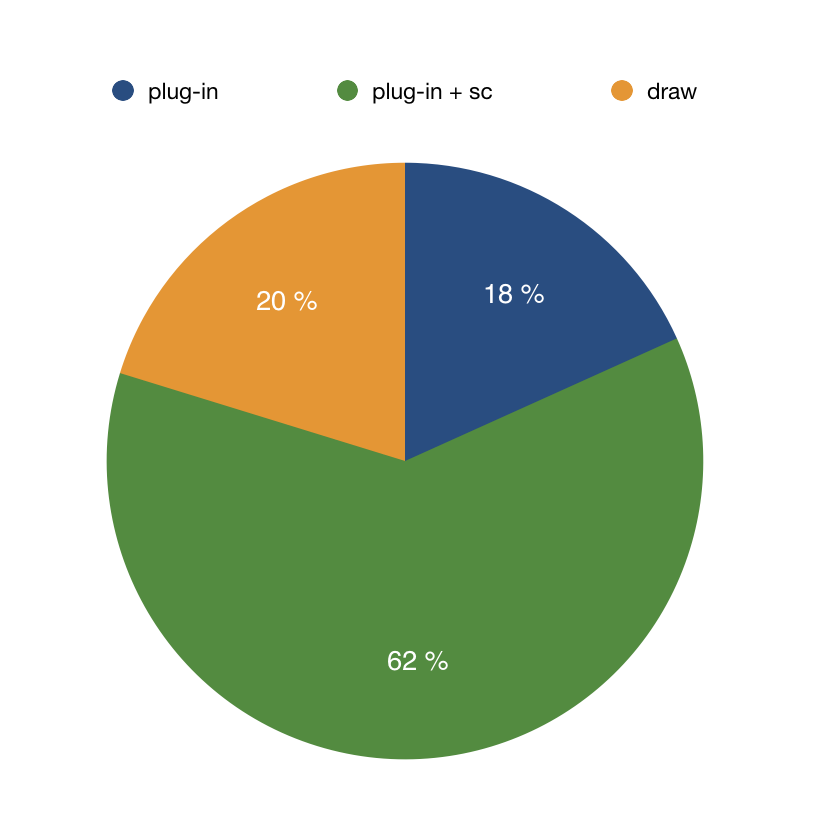
\includegraphics[width=0.55\textwidth]{images/betterRating}
\centering
\caption{Plug-in setting with better rating (all tests)}
\end{figure}

\newpage\chapter{Results}
\label{chapter:results}

The realisation of the objective could be achieved with a satisfactory result. During the process of development the JUCE Framework emphasises as a good choice by supporting with basic but solid functionality for an audio plug-in which would have been very time-consuming to build up from scratch.\\
With the first prototype version it was already possible to obtain favourable results (reasonable parameter settings implied). Nevertheless it still had some unfavorable problems and unfinished design decisions. The comparison to “Vocal Rider” approved the functionality of the prototype but also pointed out the differences between the two approaches of the plug-ins. Despite the differences the comparison resulted in ideas for further improvements of the study plug-in.\\
In retrospective view quite a lot improvements enhanced the early prototype. The additions with most influence on the plug-ins performance where the extra idle time for ignoring small breathing or rhythmic gaps between vocal signals, the ability to draw gain automations into the DAW, the side chain feature and the automatic detection of parameters.\\
The side chain feature validated its use in the according hearing test where its advantages for the plug-in where observable as well as the outcome of a plug-in with this feature enabled getting quite close to the optimal reference (which performed the gain adaption with oracle knowledge).\\

\section{Future Improvements}

The study plug-in meets the requirement of the objective but it could still be improved.\\
For example, parameter detection is an optional feature which could be useful to set the plug-in correctly, especially at first interactions of a user but as described in the corresponding chapter \ref{chapter:improvements}.2 and \ref{chapter:improvements}.3, it is only able to calculate ‘online’ during playback of the song. An offline calculation is not implemented yet which would be significantly faster. As one purpose of the plug-in is to save time for the mixing engineer, it would be great to enhance the feature with offline calculations in future development. When the offline calculation is possible it would be able to measure the perceived signal level by using the loudness algorithm\cite{ITUalgo} which may improve the plug-in’s outcome.\\
An other option of a reasonable future improvement would be to extend its scope of application. Currently it is designed to work with vocal signals but other recordings may show similar problems e.g. recordings of the bass guitar. Therefore it would be useful to have the opportunity to chose between different presets for the main constants of the plug-in’s calculation, fitting the different signals.\\
Additional to possible algorithmic improvements the plug-in could be improved by further testing for increased stability and correctness of the results.\\

\section{Conclusion}

A plug-in for decreasement of long term dynamics was developed. During the work on this study the plug-in’s prototype frequently changes and additional improvements in terms of features, algorithms and parameters were included.\\
It certainly might get further improvements in different parts but in final conclusion the study resulted in a plug-in mature enough to fulfil its intended task in daily production, and even some features more.\\




\newpage\chapter{Discussion}
\label{chapter:discussion}

In the gggg
\newpage\chapter{Conclusion}
\label{chapter:conclusion}

The realisation of the objective could be achieved with a satisfactory result. During the process of development the JUCE Framework emphasises as a good choice by supporting with basic but solid functionality for an audio plug-in which would have been very time-consuming to build up from scratch.\\
With the first prototype version it was already possible to obtain favourable results (reasonable parameter settings implied). Nevertheless it still had some unfavorable problems and unfinished design decisions. The comparison to “Vocal Rider” approved the functionality of the prototype but also pointed out the differences between the two approaches of the plug-ins. Despite the differences the comparison resulted in ideas for further improvements of the study plug-in.\\
In retrospective view quite a lot improvements enhanced the early prototype. The additions with most influence on the plug-ins performance where the extra idle time for ignoring small breathing or rhythmic gaps between vocal signals, the ability to draw gain automations into the DAW, the side chain feature and the automatic detection of parameters.\\
The side chain feature validated its use in the according hearing test where its advantages for the plug-in where observable as well as the outcome of a plug-in with this feature enabled getting quite close to the optimal reference (which performed the gain adaption with oracle knowledge).\\

\section{Future Improvements}

The study plug-in meets the requirement of the objective but it could still be improved.\\
For example, parameter detection is an optional feature which could be useful to set the plug-in correctly, especially at first interactions of a user but as described in the corresponding chapter \ref{chapter:improvements}.2 and \ref{chapter:improvements}.3, it is only able to calculate ‘online’ during playback of the song. An offline calculation is not implemented yet which would be significantly faster. As one purpose of the plug-in is to save time for the mixing engineer, it would be great to enhance the feature with offline calculations in future development. When the offline calculation is possible it would be able to measure the perceived signal level by using the loudness algorithm\cite{ITUalgo} which may improve the plug-in’s outcome.\\
An other option of a reasonable future improvement would be to extend its scope of application. Currently it is designed to work with vocal signals but other recordings may show similar problems e.g. recordings of the bass guitar. Therefore it would be useful to have the opportunity to chose between different presets for the main constants of the plug-in’s calculation, fitting the different signals.\\
Additional to possible algorithmic improvements the plug-in could be improved by further testing for increased stability and correctness of the results.\\

\section{Conclusion}

A plug-in for decreasement of long term dynamics was developed. During the work on this study the plug-in’s prototype frequently changes and additional improvements in terms of features, algorithms and parameters were included.\\
It certainly might get further improvements in different parts but in final conclusion the study resulted in a plug-in mature enough to fulfil its intended task in daily production, and even some features more.\\




\finish